The first step in the process of reconstructing the 3D geometry of the object
is to establish a mathematical relationship between the natural units of the
camera with the physical units of the 3D world. We use camera calibration to
estimate the internal parameters of the camera and its distortion coefficients.
The geometry is described in terms of camera's optical center and focal
length of the camera.

\begin{figure}[ht!]
\centering
\subfigure{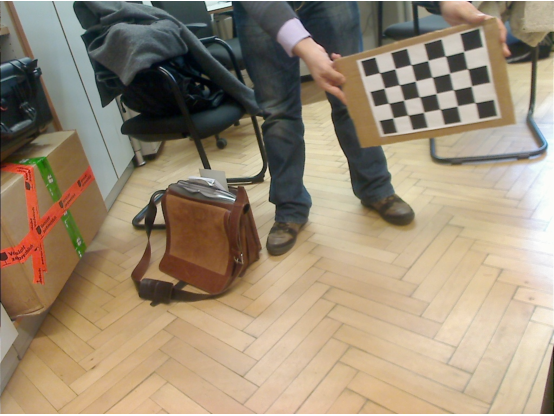
\includegraphics[width=.48\linewidth]{figures/calibrate-1}}\quad
\subfigure{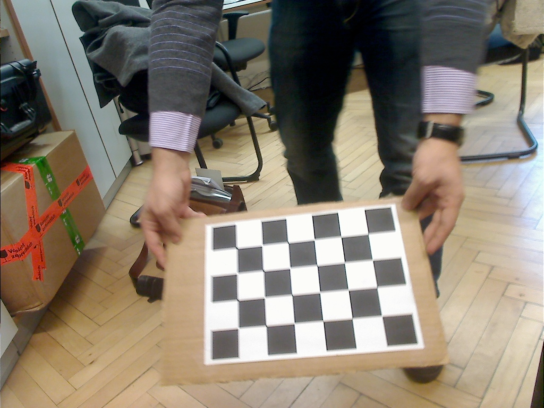
\includegraphics[width=.48\linewidth]{figures/calibrate-2}} \\
\subfigure{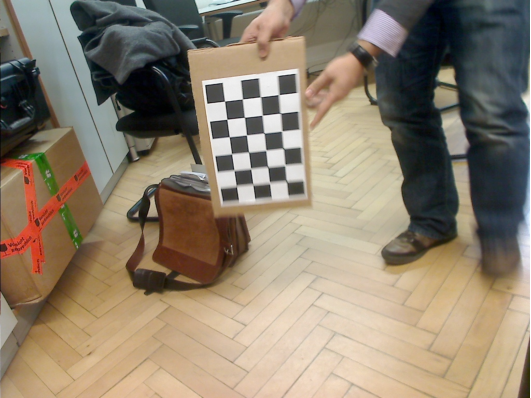
\includegraphics[width=.48\linewidth]{figures/calibrate-3}}\quad
\subfigure{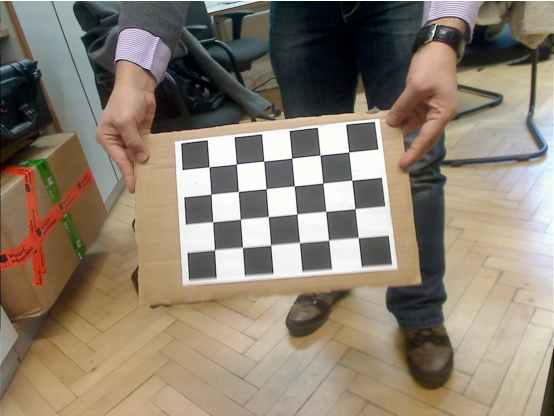
\includegraphics[width=.48\linewidth]{figures/calibrate-4}}
\caption{Calculating the Camera's Intrinsic Parameters}
\label{figure:camera-calibration-intrinsics}
\end{figure}

We use OpenCV camera calibration routines and a planar chessboard pattern as
our calibration object. OpenCV uses Zhang's method \cite{zhang:2000} to
calculate the focal lengths and offsets. However it uses Brown's method
\cite{brown:1971} to calculate the distortion coefficients. The calibration
pattern is rotated and translated to provide multiple views in order to get
precise information about the intrinsic parameters of the camera as shown in
Fig.  \ref{figure:camera-calibration-intrinsics}.  The OpenCV routine
\texttt{cvFindChessboardCorners()} is used to locate the corners and once we
have enough corners from multiple images, we use \texttt{cvCalibrateCamera2()}
to get the intrinsic matrix $A$ as shown in Eq. \ref{equation:calibrate}.

\begin{align}
	\label{equation:calibrate}
	s \times
	\begin{bmatrix}
		u \\ v \\	1 \\
	\end{bmatrix} &= A \cdot \begin{bmatrix}
															R \mid T
	 				  								\end{bmatrix}
										 \cdot \begin{bmatrix}
															x_w \\ y_w \\ z_w \\ 1
														\end{bmatrix} \\
	\text{where}~
	A &= \begin{bmatrix}
					f_x & 0 & c_x \\
					0 & f_y & c_y \\
					0 & 0 & 1 \\
 		 	 \end{bmatrix} \notag
\end{align}

The intrinsic matrix $A$ is later used to describe the pose of the object
being scanned by the laser relative to the coordinate system of the camera. In
order to determine this pose on both sides of the target object, the patterns
are masked to allow individual calculation as shown in Fig.
\ref{figure:camera-calibration-extrinsics}. The parameters represented by
$\begin{bmatrix}R \mid T\end{bmatrix}$ are then separately calculated for both
the sides by calling the OpenCV routine
\texttt{cvFindExtrinsicCameraParams2()}.

\begin{figure}[ht!]
\centering
\subfigure[$R_1 \mid T_1$]
{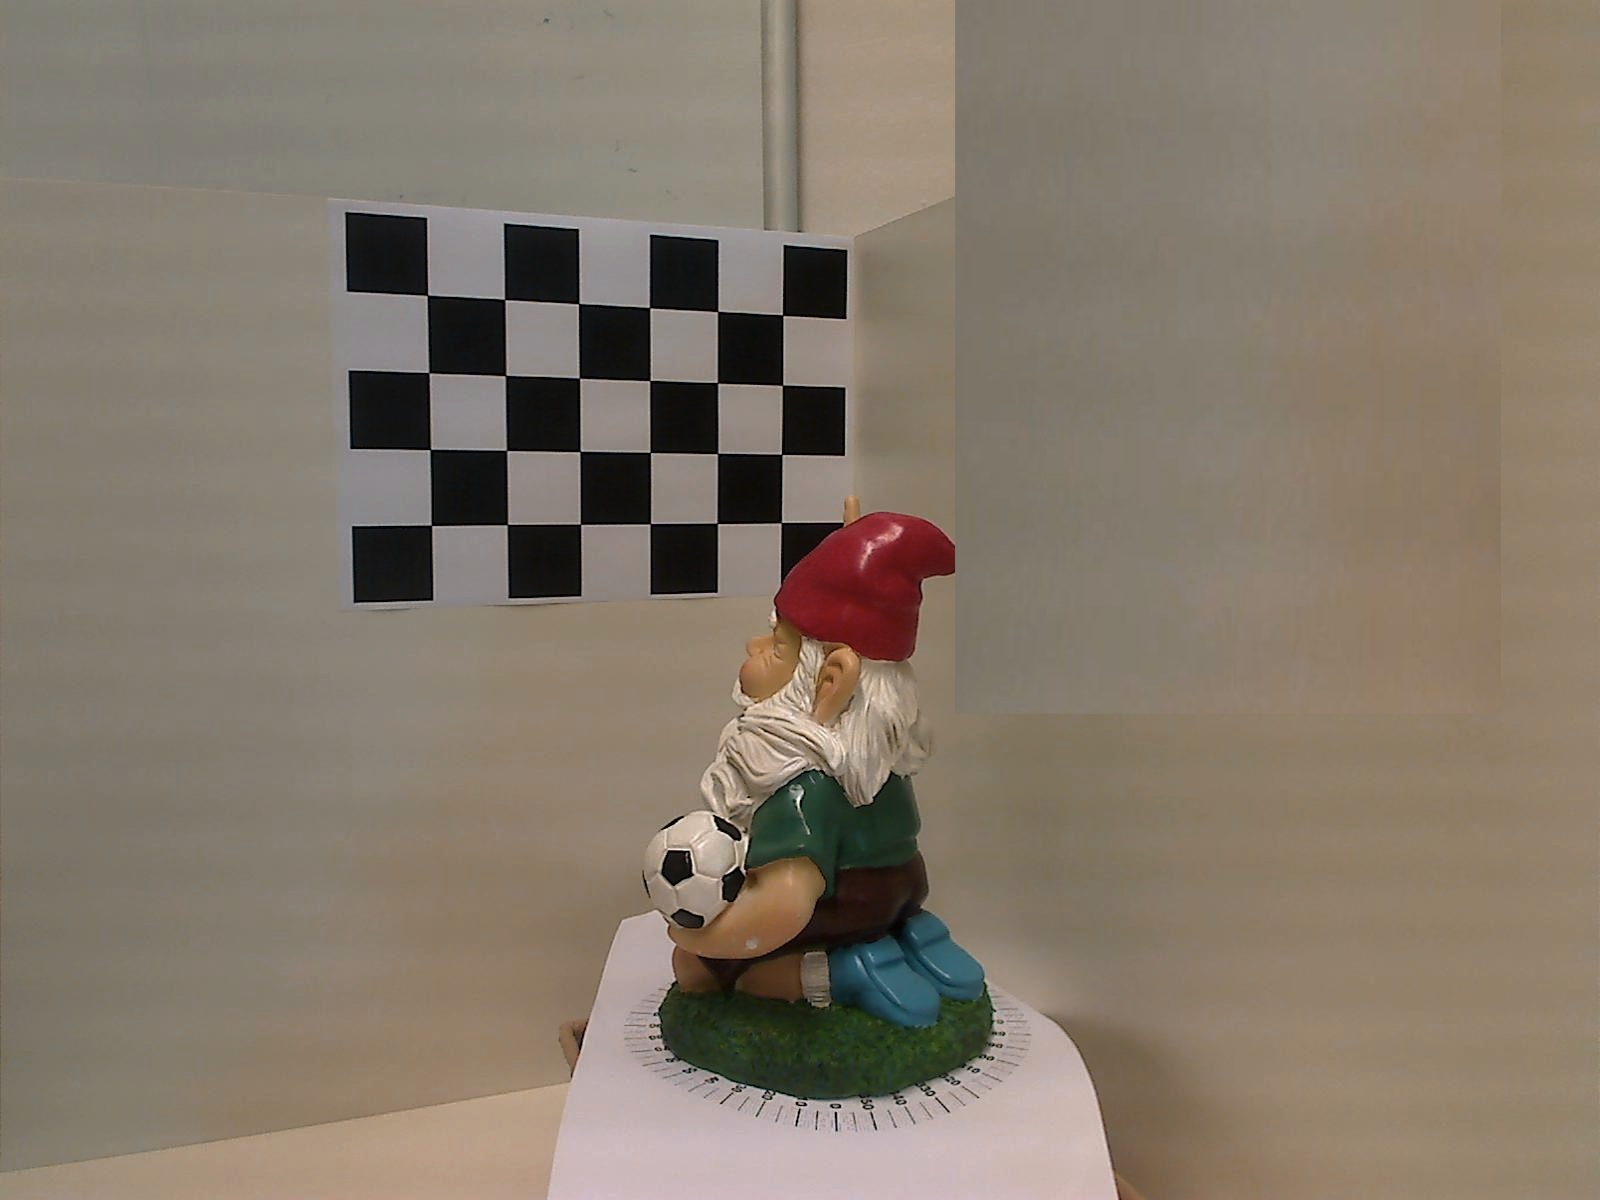
\includegraphics[width=.47\linewidth]{figures/calibrate-5}} \quad
\subfigure[$R_2 \mid T_2$]
{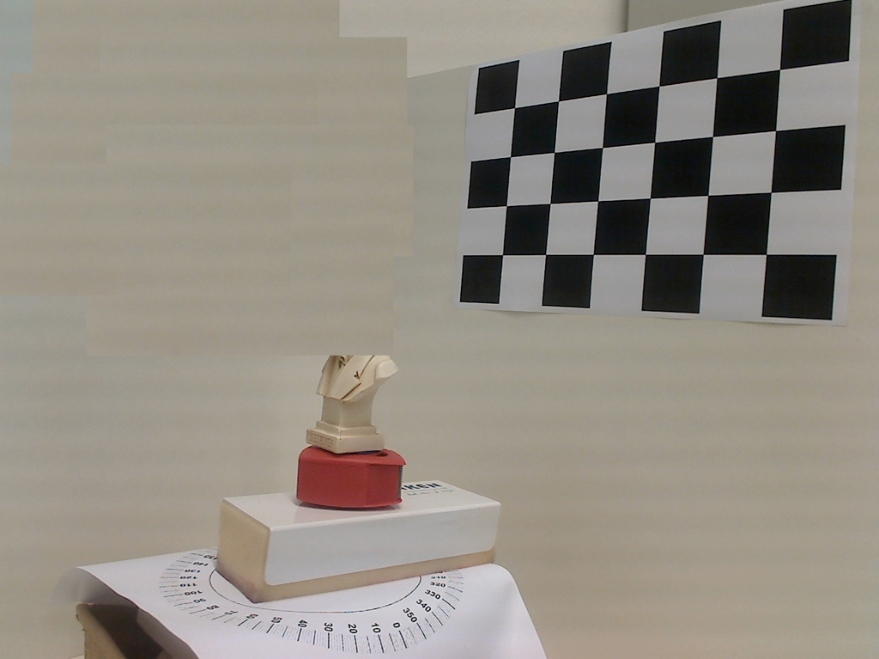
\includegraphics[width=.47\linewidth]{figures/calibrate-6}}
\caption{Calculating the Camera's Extrinsic Parameters}
\label{figure:camera-calibration-extrinsics}
\end{figure}

